%!TEX root=../main.tex
\chapter{Climbing Mont Blanc Improvements}
\label{ch:improvements}
This chapter describes the implementation of the usability and improvement goals presented in \Cref{sec:ps-inter}, as well as a short discussion of the proposal objectives presented in the same section:
\begin{itemize}
    \item Fix bugs and known issues in the system, i.e objective \texttt{U1}.
    \item Change the existing \gls{dbms} into a more sophisticated one, i.e objective \texttt{I1}.
    \item Implement and extend the \gls{cmb} system's usability features in accordance with the \gls{cmb} team, i.e objective \texttt{U2}.
    \item Propose improvements to a existing stability test, improvements to the HowTo-page and existing provided problems, and implementation of a discussion forum, i.e objectives \texttt{P1}, \texttt{P2}, and \texttt{P3} respectively.
\end{itemize}
A frontend data model is in the below sections meant by an entity which stores data. A data model does also contain control logic to modify or update stored data, and therefore also acts as a \textit{controller}. For example, fetching data from \gls{rest}ful \glspl{api} is common in the \gls{cmb} prototype frontend data models. Each model is also coupled with a frontend view, which uses the internal logic of the data model to present the model data to users.
%In this chapter it is assumed that a web interface follows the \gls{mvc} pattern. As briefly mentioned in sub-\Cref{subsec:cmb-arch-frontend}, Angular structures the HTML and Javascript code according to the \gls{mvc} pattern, and the reader should have the abstraction in mind when reading about browser or frontend implementations.
\clearpage
\section{Real Time Updates}
\label{sec:real-time}
The frontend view changes when a user performes actions against the frontend models as mentioned in Sub-\Cref{subsec:cmb-arch-frontend}. However, the frontend view presented to a given user does not update automatically as other users interact and changes their data models, as models are stored locally in each of the user’s browser. If the updated model contains data that should be known\footnote{Hereby known as \textit{shared data}.} to all users, the users does not get notified about the model changes dynamically and views may, therefore, display out of date information. Figure \ref{fig:update-problem} an example of the problem, as Alice updates some of her browser’s model data when she interacts with the system. If Alice changes some data present in Bob’s models, Bob will not be notified of the changes as all data transfer are done with HTTP requests between Alice and the server. However, Bob can fetch up to date data by manually refreshing his web page. \\

\begin{figure}
    \centering
    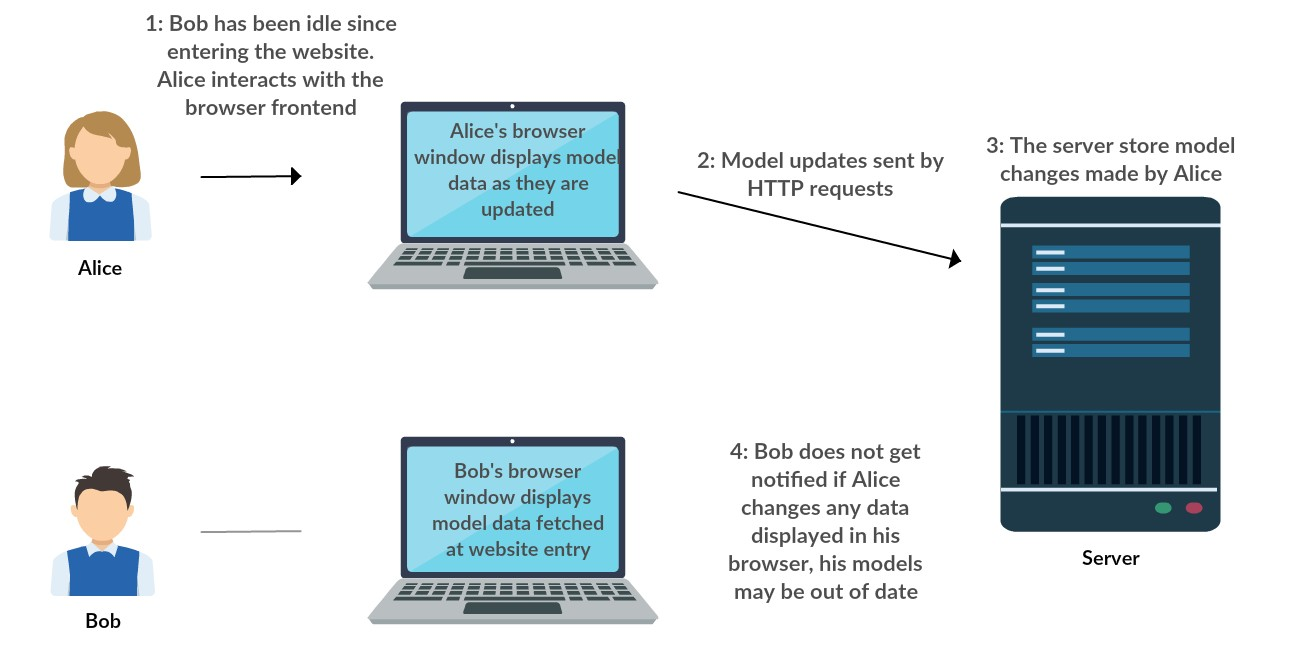
\includegraphics[width=1\textwidth]{figs/update_problem.jpg}
    \caption{Example of updating models without model change notifications}
    \label{fig:update-problem}
\end{figure}

Many websites requires to share data between multiple clients and dynamically notify clients if there are changes to the data. As an example in the \gls{cmb} system, it would be nice if the frontend interface dynamically updated as a user’s submission finished running at the backend. In the old system before the improvements, the user had to update the data manually by clicking a refresh button provided by the user interface or manually refresh the web page. However, this section presents a technology which has been introduced in the new version of the system to dynamically update data relevant for multiple clients. \\

Socket.io \cite{SOCKETIO} is an \gls{api} for enabling real-time communication between the server and connected clients. The \gls{api} was first made as Javascript library, but many open source projects have developed modules for other programming languages integrating the \gls{api}. One benefit of the \gls{api} is that it works as a wrapper around a set of real-time communication protocols to enable support for different browsers, which means that the framework can automatically detect the protocol supported by a client and use that information to select the best-fitted communication protocol. \\

Rohit Rai states the communication protocols supported by the Socket.io \gls{api} \cite{Rai2013}. As many protocols are available, Figure \ref{fig:cmb-protocols} only shows the communication protocols enabled in the new version of \gls{cmb}. The WebSocket protocol \cite{a:Fette2011}, shown in Figure \ref{fig:websocket}, has become more popular since its introduction in 2011 and is now supported by the most popular browsers. The protocol is a bit different from the well known HTTP protocol, as there is a persistent connection, or socket, between the client and the server as long as both entities are connected to the socket. The socket connection is closed if the client closes the browser window or the server goes down, or if the code explicitly indicates to close the socket. WebSockets enables easy two-way communication by letting two entities emit (read: send) messages back and forth on the socket connection and respond differently depending on the type of message emitted on the socket. \\

Polling and long-polling both use the HTTP protocol and may seem similar at first glance. However, in long-polling, the server keeps the connection between the two entities open until there is an update to the requested data as shown in Figure \ref{fig:long-polling}. In polling, as shown in Figure \ref{fig:polling}, the client continuously requests data with some constant delay between each request, while the server respond on each request with the data currently stored at the server. To make the below discussions more explainable, we can think of the connection between the server and the client as a "socket" which is a persistent communication channel with the same functionality for each of the presented protocols. \\

\begin{figure}
    \centering
    \begin{subfigure}[b]{1.0\textwidth}
        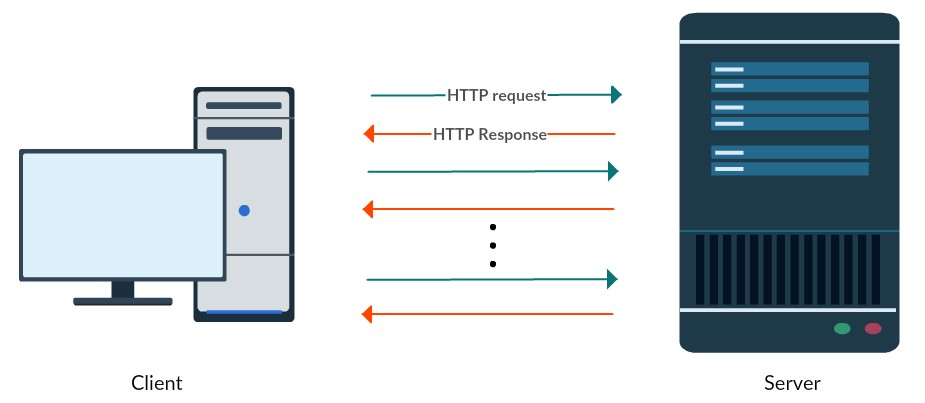
\includegraphics[width=\textwidth]{figs/polling.jpg}
        \caption{Polling: The client sends a series of HTTP request and the server responds on each request.}
        \label{fig:polling}
    \end{subfigure}
    ~ %add desired spacing between images, e. g. ~, \quad, \qquad, \hfill etc.
    %(or a blank line to force the subfigure onto a new line)
    \begin{subfigure}[b]{1.0\textwidth}
        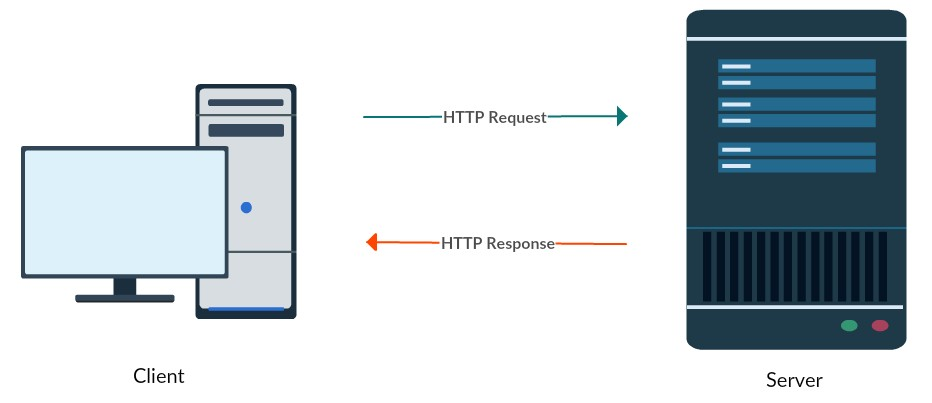
\includegraphics[width=\textwidth]{figs/long_polling.jpg}
        \caption{Long-polling: The client sends an HTTP request to fetch new data, the server holds the connection open until the requested data is updated.}
        \label{fig:long-polling}
    \end{subfigure}
    \begin{subfigure}[b]{1.0\textwidth}
        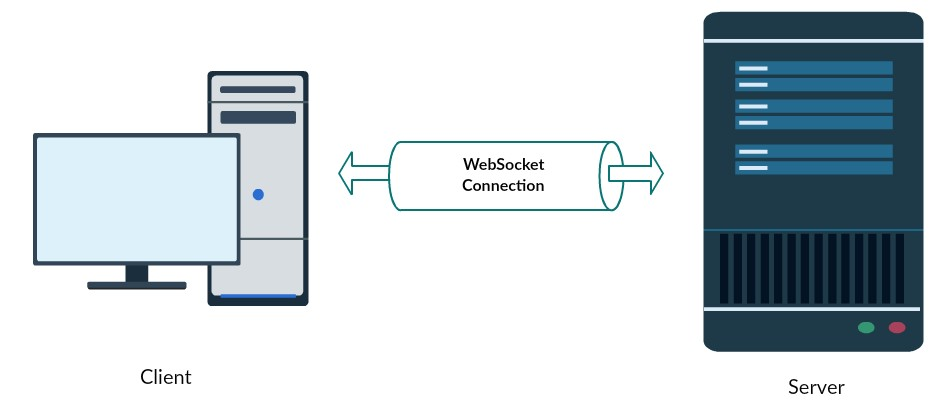
\includegraphics[width=\textwidth]{figs/websocket.jpg}
        \caption{WebSocket protocol: a two-way connection tunnel open throughout the whole client session. TCP is used as a transport protocol.}
        \label{fig:websocket}
    \end{subfigure}
    \caption{\gls{cmb} Socket.io communication protocols}\label{fig:cmb-protocols}
\end{figure}

Each socket can be "\textit{namespaced}" into separate communication channels within an application. A namespace can be viewed as an endpoint or network path, for example in the new \gls{cmb} prototype the namespace \textit{/cmb} is used as default namespace to emit messages between the client and the server. Every client initiating a socket on the namespace receives all messages emitted to the namespace, which makes it easy to share information between the server and clients connected to the namespace. \\

Each namespace can also define a set of \textit{rooms}, which can be viewed as sub-channels of a given namespace. A client needs to join a room explicitly to receive the messages emitted within a sub-channel. Figure \ref{fig:namespaces-and-rooms} illustrates the concept. Each message emitted to the namespace \textit{/cmb} are received by both client one and two. Client three will only receive those messages emitted to the namespace \textit{/test}. If a message is emitted to room one within the \textit{/cmb} namespace, only client one will receive the message. \\

Socket.io also lets the programmer define \textit{events}, which can be emitted between the server and connected clients. Table \ref{tab:cmb-socketio-events} shows the events currently defined for the \gls{cmb}, and the actions taken either by the server or client depending on which entity that emitted the event. The actions are only taken if the code defines event listeners for each event, and for the frontend, it depends on the view that is displayed in each users’ browser. As an example, the submission events shown in Table \ref{tab:cmb-socketio-events} are only valid if a given user is viewing the problem-screen shown in Figure \ref{fig:problem-view}. This makes sense because we are trying to do real-time updates to the highscore-list and the user’s submissions while he or she stays in the problem screen. Events will therefore not be received if the users navigates to another view, as Socket.io event listeners in the frontend code are bound to views or rather the views’ controllers.  \\

The two sub-sections below describes the technologies used by the server and frontend  to support real-time communication with Socket.io.

\begin{table}[t!]
    \centering
    \begin{tabular}{ | c | c | c | p{3.5cm} | }
    \hline
    \textbf{Event Name} & \textbf{Emitted by} & \textbf{Received by} & \textbf{Action}\\
    \hline
    \textit{join-problem} & Client(s) & Server & Server adds the client to the problem room specified in the emitted message. \\ \hline
    \textit{leave-problem} & Client(s) & Server & Server removes the client from the problem room specified in the emitted message. \\ \hline
    \textit{submission-deleted} & Server & Client(s) & Client fetches updated submission data from the server. \\ \hline
    \textit{submission-enqueued} & Server & Client(s) & Client displays a message in the browser window, notifying about queue size and information present in the emitted message. \\ \hline
    \textit{submission-dequeued} & Server & Client(s) & Client displays a message in the browser window, notifying about queue size and information present in the emitted message. \\ \hline
    \textit{submission-finished} & Server & Client(s) & Client loads own submissions as well as possible updates to the highscore list. \\ \hline
    \end{tabular}
    \caption[\gls{cmb} Socket.io events and corresponding actions]{\gls{cmb} Socket.io events and corresponding actions. Each submission event is sent to a room which simply is the database id of a given problem. Since we have one room per problem, we know that all submission events within a room have information about submissions made to a given problem. Remember that client views need to define event listeners to take action upon events, and in our case, the submission events above are only defined in the problem view.}
    \label{tab:cmb-socketio-events}
\end{table}

\begin{figure}
    \centering
    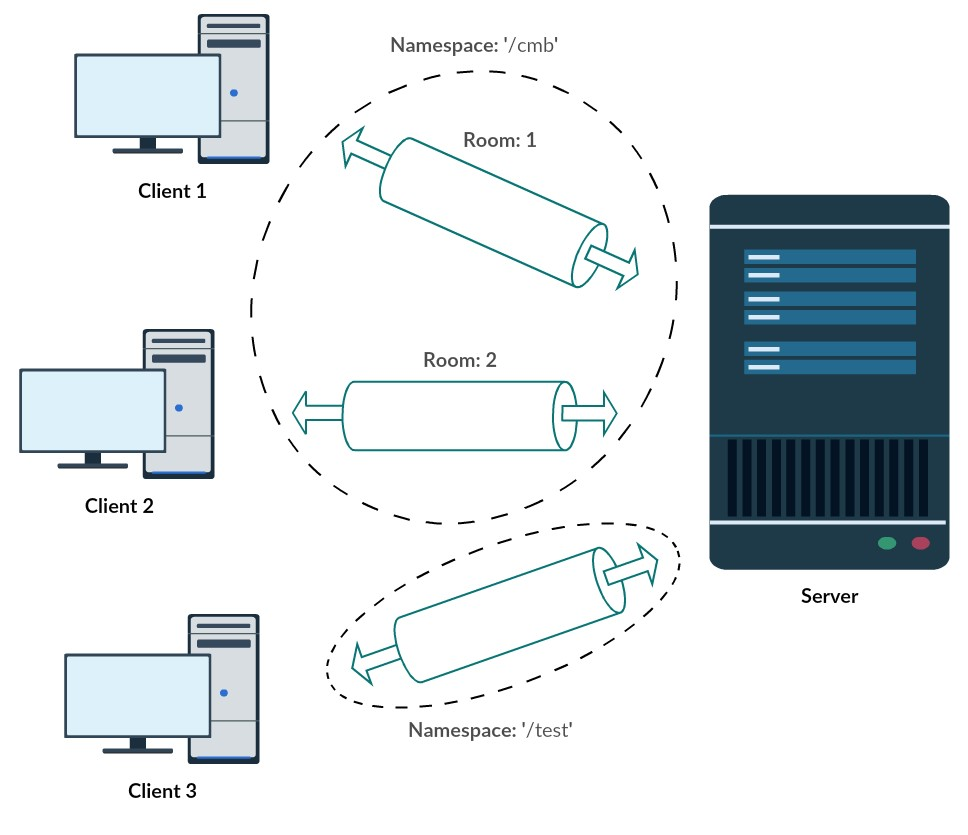
\includegraphics[width=0.87\textwidth]{figs/namespaces_and_rooms.jpg}
    \caption[Socketio namespaces and rooms in the \gls{cmb} system]{Socketio namespaces and rooms in the \gls{cmb} system. }
    \label{fig:namespaces-and-rooms}
\end{figure}

\begin{figure}
    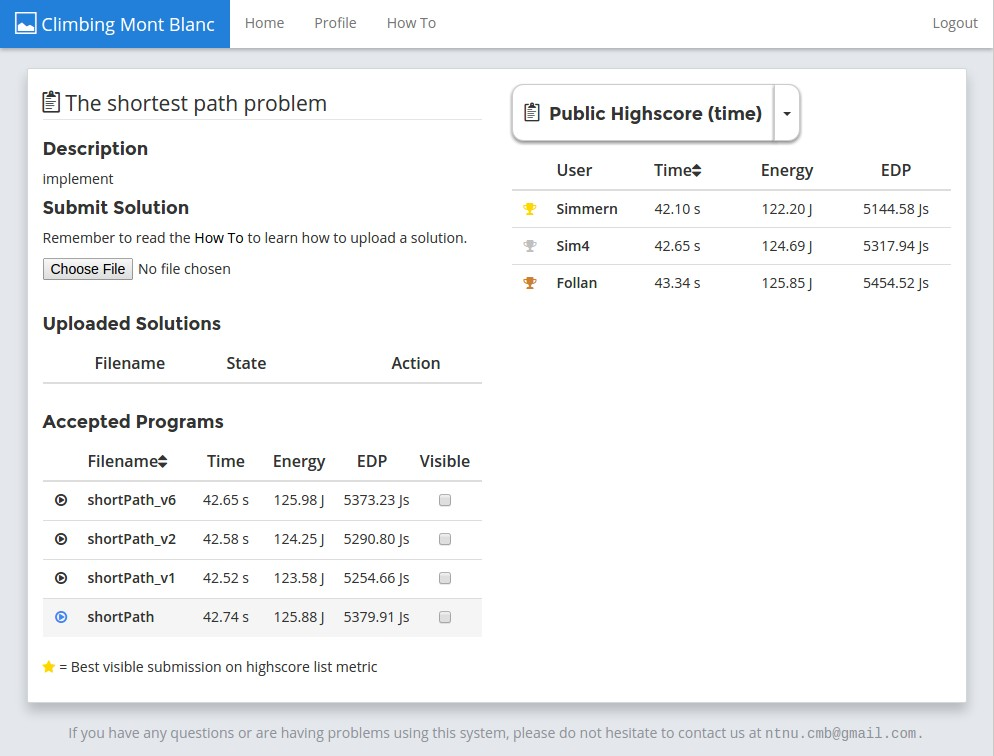
\includegraphics[width=1.0\textwidth]{figs/problem_view.jpg}
    \caption[The updated problem-view]{The updated problem-view.}
    \label{fig:problem-view}
\end{figure}

\subsection{Frontend Technology}
\label{sub-sec:real-time-frontend}
The frontend uses the client Socket.io library \cite{SOCKETIO} through an existing Angular component called \texttt{angular-socket-io} provided by Brian Ford \cite{ANGULARSOCKETIO}. The component is used to define an Angular \textit{factory}, which is simply a component that gathers and structures the setup of Socket.io in the client into a single service. The defined factory can then be used by other components in the Angular app, by marking components as a dependency of the Socket.io factory. \\

\subsection{Server Technology}
\label{sub-sec:real-time-server}
The Python module Flask-SocketIO \cite{FLASKSOCKETIO} enables Flask applications to use the SocketIO \gls{api}. Also, the modules gevent \cite{GEVENT} and gevent-websocket \cite{GEVENTWEBSOCKET}  is installed in combination with the Socket.io module to enable the use of the WebSocket protocol. Gevent is a coroutine-based networking library providing a high-level synchronous API on top of an asynchronous webserver. Asynchronous coroutines are used to handle multiple concurrent requests from multiple clients and is required by the Flask-SocketIO module to support the WebSocket transport. \\

To fully support the WebSocket protocol Gunicorn also needs to make use custom gevent worker supporting the WebSocket protocol. As stated by Miguel Grinberg on the Flask-Socketio documentation website, Gunicorn can only enable one worker due to limitations in the implemented load balancing algorithm. The Gunicorn load balancing algorithm cannot simply handle multiple workers and persistent WebSockets connections, which limits us to one worker per server. However, the worker uses coroutines to handle multiple concurrent requests as stated above. The gevent worker is enabled on the development server of \gls{cmb}, which also required some changes to the Nginx setup to entirely support the WebSocket protocol. Appendix \ref{apdx:setup} describes setup information necessary to setup servers with Gunicorn and Nginx, while \Cref{sec:eval-tech} discusses pros and cons with selected technologies as well as presenting alternatives to the selected technology stack.

\section{Frontend}
\label{sec:impr-frontend}
This section will present figures of the views in the frontend that have changed in the new version of the system. Appendix \ref{apdx:theory} shows screenshots of the old system frontend for comparison. The below sub-sections will explain the improvements and updates done to the listed views. The other views in the system are not listed here as their functionality nor appearance has changed drastically but have rather been changed to keep the views’ styling consistent throughout the system.

\begin{figure}[h!]
    \centering
    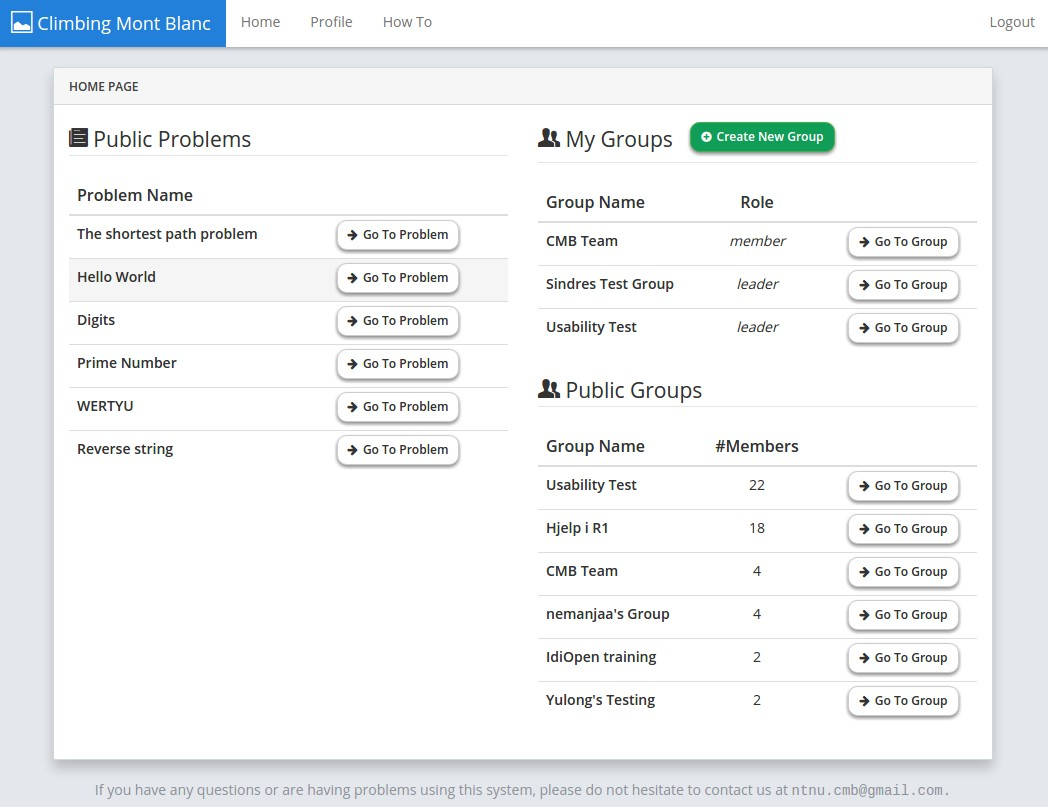
\includegraphics[width=0.7\textwidth]{figs/new_homepage.jpg}
    \caption[The updated leader view]{The updated leader view.}
    \label{fig:new-homepage}
\end{figure}

\begin{figure}[h!]
    \centering
    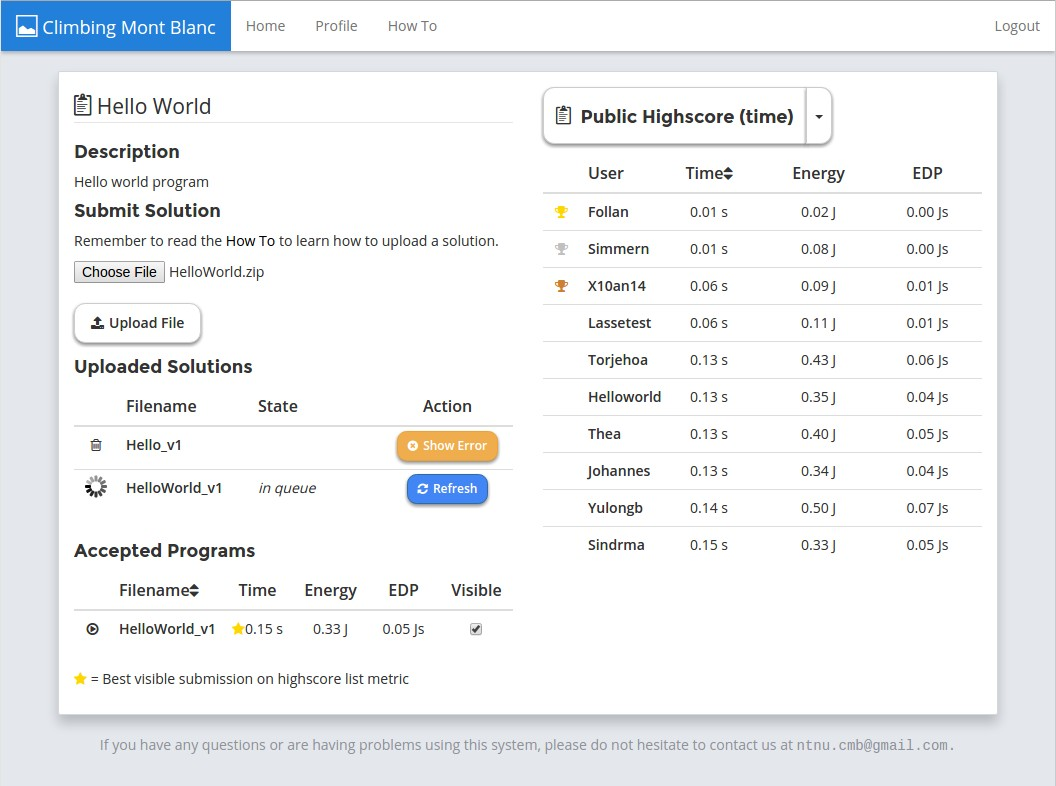
\includegraphics[width=0.7\textwidth]{figs/new_problem.jpg}
    \caption[The updated problem view]{The updated problem view.}
    \label{fig:new-problem}
\end{figure}

\begin{figure}[h!]
    \centering
    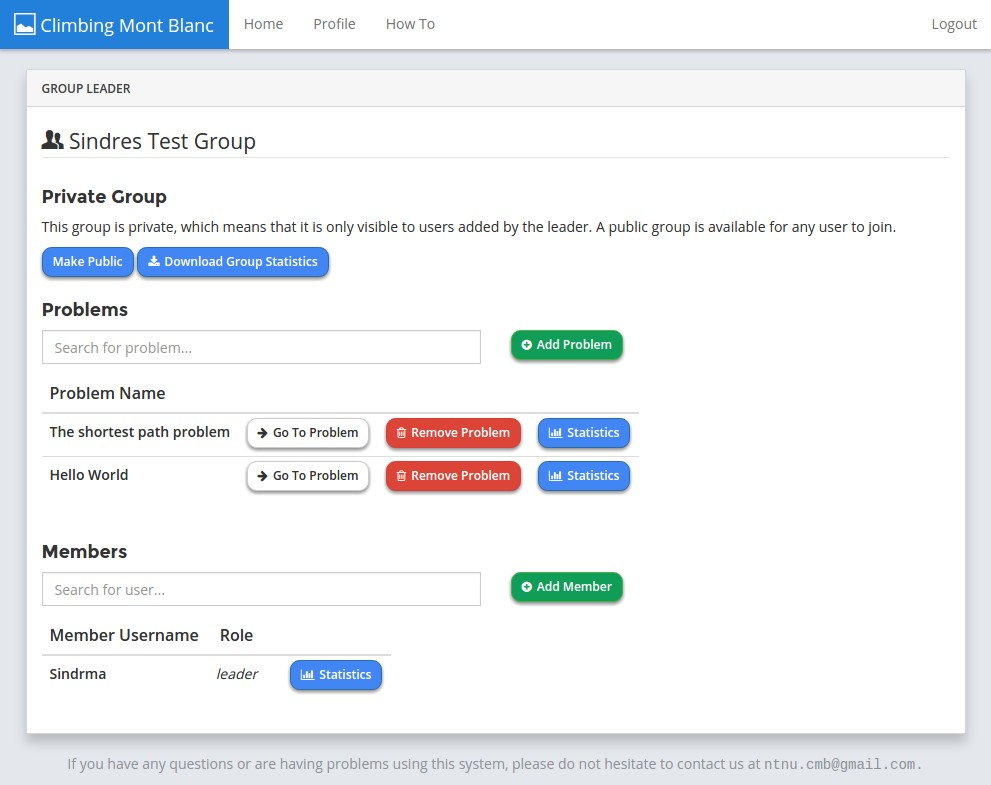
\includegraphics[width=0.7\textwidth]{figs/new_leader.jpg}
    \caption[The updated group leader view]{The updated group leader view.}
    \label{fig:new-leader}
\end{figure}

\begin{figure}[h!]
    \centering
    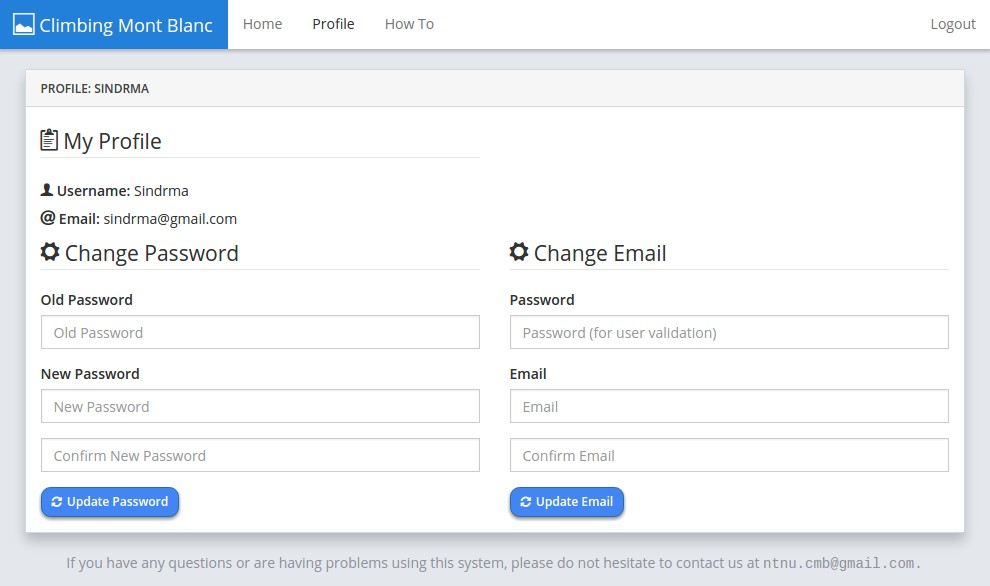
\includegraphics[width=0.7\textwidth]{figs/new_profile.jpg}
    \caption[The updated profile view]{The updated profile view.}
    \label{fig:new-profile}
\end{figure}

\subsection{Bug Fixes}
\label{sub-sec:impr-frontend-bug}
Feedback from previous user testing showed that Apple OSX users were unable to upload files to the system. The system requires the user to compress a folder containing all the source files, which has confused some users. However on OSX, users who seemingly constructed a correct zip still were unable to submit files to the system. It turned out that the most regular way of creating zip files on OSX also sometimes generated a hidden directory called \textit{\_\_MACOSX} within the zip-file. This made the upload fail, as the server assumes it receives a single compressed folder, and not multiple directories in a single zip. The users were also presented with an error message which contained little information about what went wrong. \\

The upload bug is removed in the new system. Before the zip file is sent to the server, the frontend ensures that the zip file has the required format as described above. The scan also removes all files that are not source or header files and ensures that the zip only contains a single directory containing the source files. The directory \textit{\_\_MACOSX} is also automatically removed if present in the zip. If a user tries to upload zip files with a different format than the format described above, they are presented with an error message telling them to learn more about uploading on the HowTo-page. \\

The problem view shown in Figure \ref{fig:new-problem} also contained a bug in the highscore list. When sorting on different metrics, hidden submission present in the fetched submissions would suddenly appear in the highscore list. The bug is fixed in the new system and ensures that hidden submissions are filtered out when the highscore-list is sorted on the different metrics used by the system.

\subsection{Views and Feedback}
The views in the new system have an updated styling. The home-page view shown in Figure \ref{fig:new-homepage} has a simpler table design and has removed unnecessary information, such as database ids, present in the old system. All screens containing tables has been updated according to the new table design. The problem-view shown in Figure \ref{fig:new-problem} has changed drastically compared to the old view. In the old problem-view, users needed to scroll to the bottom of the view to check out the highscore list. In the new view, the problem description and file upload functionality is vertically aligned with the highscore list, which makes it easy for users to locate the highscore list when entering the view. The old view also had a single table containing all uploads made by a user, while the new view splits the old upload table into a “Uploaded Solutions” and “Accepted Submissions” table. The table “Accepted Submissions” contains all submissions marked as finished and successful, while the rest of the submissions are shown in the “Uploaded Solutions” table. Having two tables makes the upload information more structured, and the user can quickly find information about submissions. \\

The old system displayed info and error messages in the lower right corner of the screen. The messages are very small, and can sometimes be hard to spot as they are only visible for short period of time. Since all messages also have the same styling, it is hard to differentiate between message types. An example of the old message component is shown in Figure \ref{fig:old-message}. The new system displays messages right below the navigation bar as shown in Figure \ref{fig:new-message}, which makes messages easy to spot. The messages are also split into the four message types \textit{info}, \textit{success}, \textit{danger}, \textit{error}, and each message type has their own color as shown by Figure \ref{fig:type-color}. Error messages have also been updated with more descriptive messages if needed. \\

\begin{figure}[h!]
    \centering
    
\includegraphics[width=0.5\textwidth]{figs/old_message.jpg}
    \caption[Example of an old popup feedback message]{Example of an old popup feedback message}
    \label{fig:old-message}
\end{figure}


\begin{figure}[h!]
    \centering
    \begin{subfigure}[b]{0.48\textwidth}
        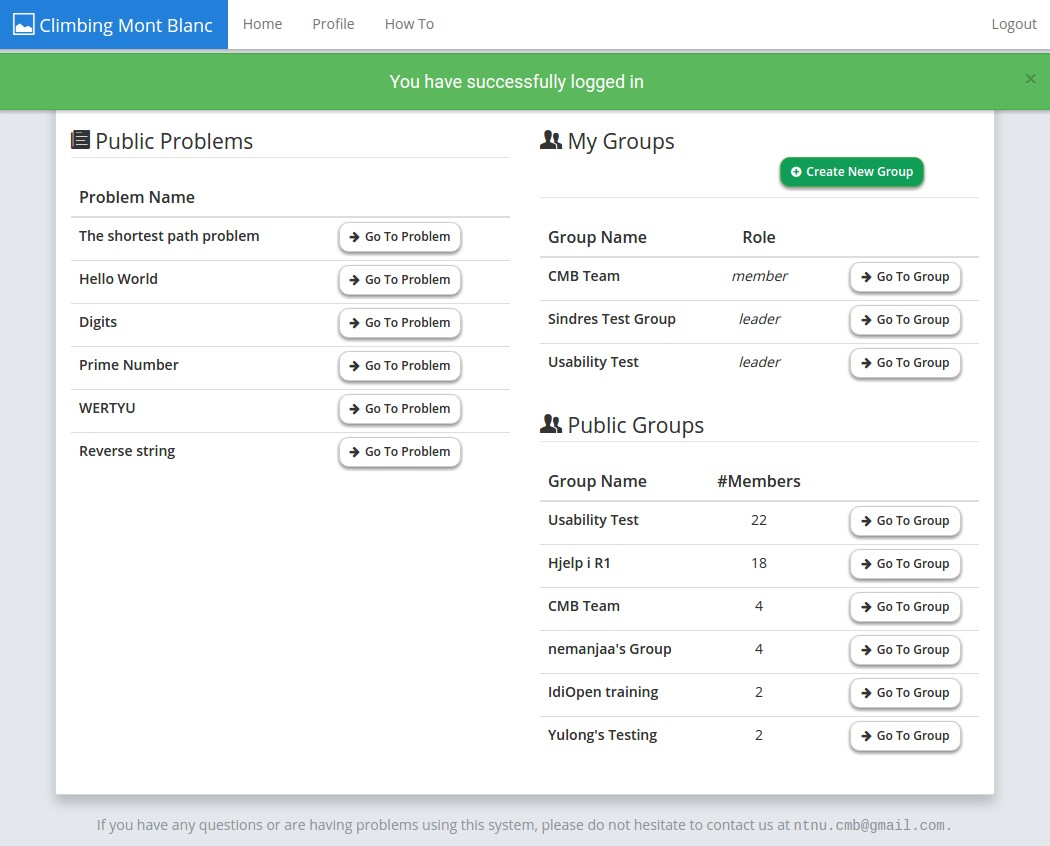
\includegraphics[width=\textwidth]{figs/new_message.jpg}
        \caption{Example of view displaying new feedback message.}
        \label{fig:new-message}
    \end{subfigure}
    ~ %add desired spacing between images, e. g. ~, \quad, \qquad, \hfill etc.
    %(or a blank line to force the subfigure onto a new line)
    \begin{subfigure}[b]{0.48\textwidth}
        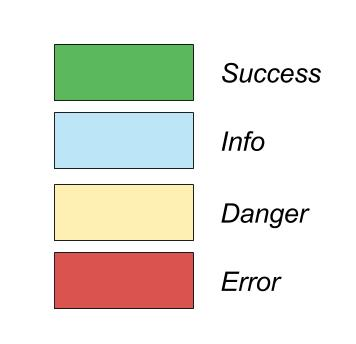
\includegraphics[width=\textwidth]{figs/type_color.jpg}
        \caption{The color of each of the defined message types}
        \label{fig:type-color}
    \end{subfigure}
    \caption{\gls{cmb} feedback messages}
    \label{fig:new-feedback}
\end{figure}
Most buttons in the new frontend also have symbols inside buttons. Symbols were added to more clearly state the purpose of the button and thereby improve usability. As an example, the problem view includes a ``play''-symbol inside the ``Run Program''-button upon successfully uploading a zip-file. The same ``play''-symbol is included in the ``Accepted Submission'' table to rerun submissions, which improves \textit{learnability} and \textit{memorability}. \\

The old system also required users to through a two-stage sequence to compile and run a program. The procedure has been further simplified into a single action in the new system, which makes the action of running a program simpler and more logical. Other buttons in the new interface have symbols as well, for example, a navigation button from the homepage to a problem view includes a right arrow to indicate movement \textit{to} a certain view. Users can thereby infer that a backward arrow means navigating back to the previous view if such a button is displayed in the system. \\

The new problem view also displays spinners on submissions currently running or in queue. An example of an active spinner on a submission in the ``Uploaded Solutions''-table shown in Figure \ref{fig:new-problem}. The table also includes the state of the submissions, which is updated in real-time as the program executes. The state field real-time updates is possible due to the real-time improvement explained in \Cref{sec:real-time}. If an error occurrs during program execution, it is possible to view the error in a popup window, or more technically a \textit{modal}, as shown in Figure \ref{fig:error-modal}. The content of the modal depends on the type of error and Table \ref{tab:error-types} shows the different error types which can occur during a program's execution. The content of the modal are decided by the ``detailed\_state'' database field in the Submissions table, which is explained in section  \ref{sec:impr-server}. The old system had an own view displaying error messages which navigated the user away from the problem view, however, in the new frontend, users stay within the problem view removing an uneccassary navigation stage. \\

\begin{figure}
    \centering
    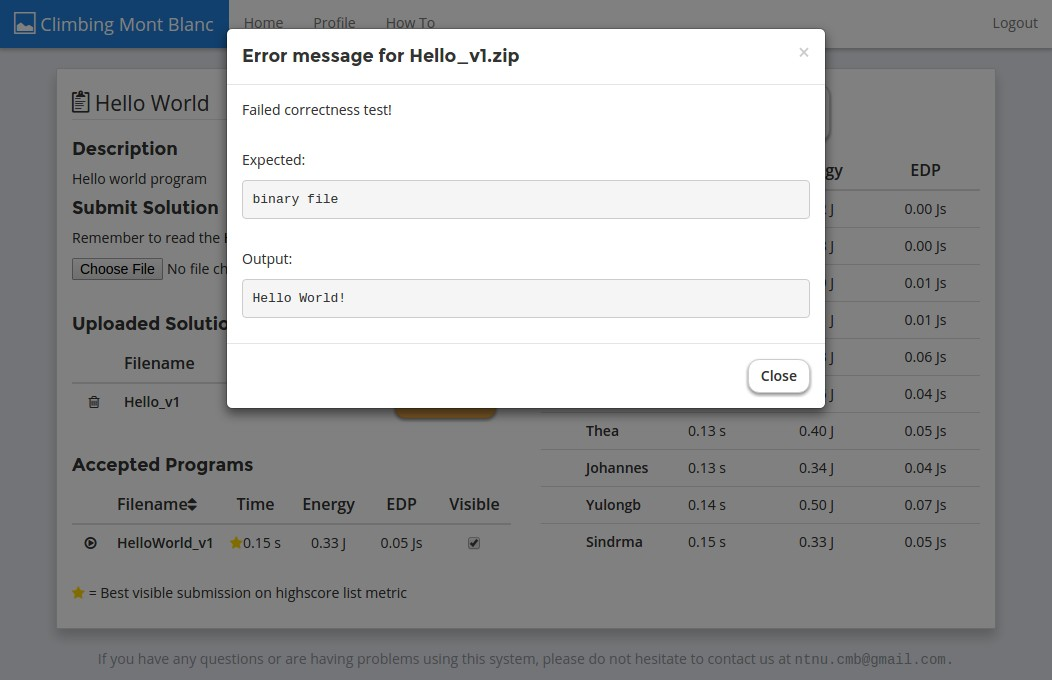
\includegraphics[width=0.7\textwidth]{figs/error_modal.jpg}
    \caption[Error modal example]{Error modal example}
    \label{fig:error-modal}
\end{figure}

\begin{table}[t!]
    \centering
    \begin{tabular}{  l | p{5.5cm}  }
    \hline
    \multicolumn{2}{  c  }{\textbf{ERROR TYPES}} \\
    \hline
    \textit{CORRECTNESS\_TIMEOUT} & A timeout occured during small correctness test. \\ \hline
    \textit{CORRECTNESS\_RUNTIME\_ERROR} & A runtime error occured during the small correctness test. \\ \hline
    \textit{CORRECTNESS\_BAD\_OUTPUT} & Output from the small correctness test was not accepted by checker. \\ \hline
    \textit{PROGRAM\_TIMEOUT} & A timeout occured during big correctness test. \\ \hline
    \textit{PROGRAM\_RUNTIME\_ERROR} & A runtime error occured during the big correctness test. \\ \hline
    \textit{PROGRAM\_BAD\_OUTPUT} & Output from the big correctness test was not accepted by checker. \\ \hline
    \end{tabular}
    \caption{\gls{cmb} error types}
    \label{tab:error-types}
\end{table}


A bulletin board displaying administrator generated messages have also been added to the frontend. Figure \ref{fig:bulletin-view} shows an example of how active bulletins looks like in the system frontend, with both removable and non-removable bulletins. \Cref{sec:impr-server} explains the server extensions made to the server code to support the bulletin board feature.

\begin{figure}[t!]
    \centering
    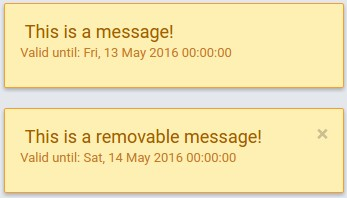
\includegraphics[width=0.5\textwidth]{figs/bulletin_view.jpg}
    \caption[Bulletin board frontend examples]{Bulletin board frontend examples}
    \label{fig:bulletin-view}
\end{figure}

\subsection{Group Functionality Improvements}
Figure \ref{fig:new-leader} shows the updated group leader view. The view is displayed if users are navigating to a given group from the homepage and is marked as the leader of the group in the database, as in the old system. Among the visual improvements mentioned in the above sub-section, the view has an extra button. The button lets the leader of a group download a \gls{json} file, which contains information about group members as well as submissions made to problems registered on the group. The file can be used to generate group statistics, which is done by
JSON stat file download. The functionality was added due to a master thesis of two students, assessing the \gls{cmb} system's suitability for conducting digital exams in the course TDT4102 Procedural and Object-Oriented Programming \cite{TDT4102}, and were needed as part of the digital exam experiment with the \gls{cmb} system. \\

The new homepage view has been extended with a ``Create New Group''-button. The button has been moved from the old profile view into the new homepage view, as users may not associate adding groups with profile information and it also gathers group information and functionality, which makes it easier to locate components related to groups in the system. The new profile view is shown in Figure \ref{fig:new-profile}.

\section{Server}
\label{sec:impr-server}
\subsection{Database Management System Updates}
\label{sub-sec:impr-dbms}
The old version of \gls{cmb} used SQLite \cite{SQLITE} as \gls{dbms} at both the development and production server. SQLite is a lightweight \gls{dbms}, which requires minimal configuration before use and is popular to use during automatic unit testing, which also is done in the \gls{cmb} system. The initial goal was to improve, and thereby possibly change, the \gls{dbms} into a more sophisticated system. However, during the Spring the \gls{cmb} team found it unnecessary to change the \gls{dbms} of performance reasons and we found it more important to extend the system with new features. \\

Unrelated to the performance reasons, a new \gls{dbms} was wanted by the \gls{cmb} team and the IDI Department. We, therefore, changed the \gls{dbms} to MySQL due to its usage in other applications developed at the IDI Department. IDI provided the databases used by the system, and we also gained access to a database administrator interface available at \url{https://phpmyadmin.idi.ntnu.no/}. SQLAlchemy made the switch onto the new \gls{dbms} easy as it has a predefined MySQL adapter and had no problems in setting up the new databases for our development and production servers. Further, Flask-Migrate \cite{FLASKMIGRATE}, used for database \textit{migrations}\footnote{Database migration is the task of managing versions of a database schema without altering previously stored database content.}, also worked without any changes in configuration. \\

A complete database dump was made from the SQLite databases. All SQL \texttt{INSERT} statements in the database dump were extracted and executed against the new development and production databases, to move all previously stored data in the SQLite databases over to the MySQL databases. The actions were performed with a combination of terminal commands and the database admin interface provided by IDI. MySQL and SQLAlchemy have not had any performance issues in the IDI Department, so the system uses the standard MySQL adapter provided by SQLALchemy. Implementing and enabling non-blocking database access has been added back to the backlog found in Appendix \ref{apdx:backlog} as a performance improvement.

\subsection{Database Schema Updates}
\label{subsec:impr-database}
The updates to the previous database schema are shown in Figure \ref{fig:updated-database-schema}. The Submissions-table have been updated with two new fields. The ``detailed\_state'' field was added to provide more information about a run to the user. In the current improved system, it contains a detailed string about a submissions state as it returns from the backend as explained in \Cref{sec:impr-backend}. The field can be modified in the future to store \gls{json} instead of simple text if more information about a submission becomes available when executing code on the backend. \textit{Future developers should strive against always keeping users up-to-date with the state of their submissions}, and the new field aims to enable such feedback as explained in \Cref{sec:impr-frontend} above. \\

\begin{figure}
    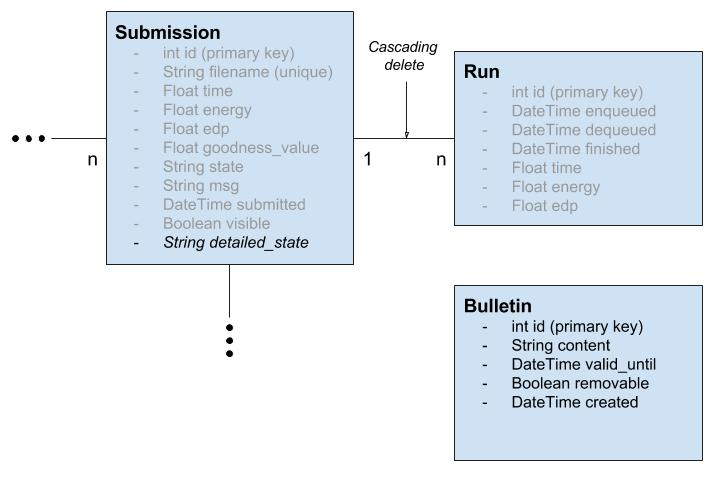
\includegraphics[width=0.9\textwidth]{figs/updated_database_schema.jpg}
    \caption[Database schema updates]{Database schema updates. The figure does only include the tables that are updated. Added table columns are highlighted. }
    \label{fig:updated-database-schema}
\end{figure}

A Bulletin-table were added to enable administrators to notify users about news and system messages. Bulletins has a field called ``valid\_until'' which indicates until which date a given bulletin is valid, and the field is used to select the valid bulletins as explained in the below sub-section and is also displayed in the frontend as explained in \Cref{sec:impr-frontend} above. Another field called ``removable'' indicates if a bulletin should be removable or not, and if the bulletin is marked as removable the user are allowed to remove the bulletin from the frontend view. \\

Cascading deletes has also been added between the Submission- and Run-tables. Cascading deletes ensures that all rows in the Run table associated with a Submission row get deleted upon deletion of a submission, which ensures that there are no dangling rows in the Run table, and the database are left in a consistent state after deleting submissions. Database consistency is of importance for both administrators and users, as both user groups can delete submissions.

\subsection{Endpoint Updates}
\label{sub-sec:impr-server-endpoint}
The routes that has been updated or added to the \gls{rest}ful \gls{api} is listed in Table \ref{tab:cmb-updated-routes}. Figure \ref{fig:postman-request} shows an example GET-request against one of the routes defined in the table, which fetches data from a local server. The table does not include changes made to \gls{api} routes due to the implementation of the real-time update improvement explained in \Cref{sec:real-time}, as the improvements do not change the internal logic of the original routes and has only added code to emit events. \\

\begin{figure}[h!]
    \centering
    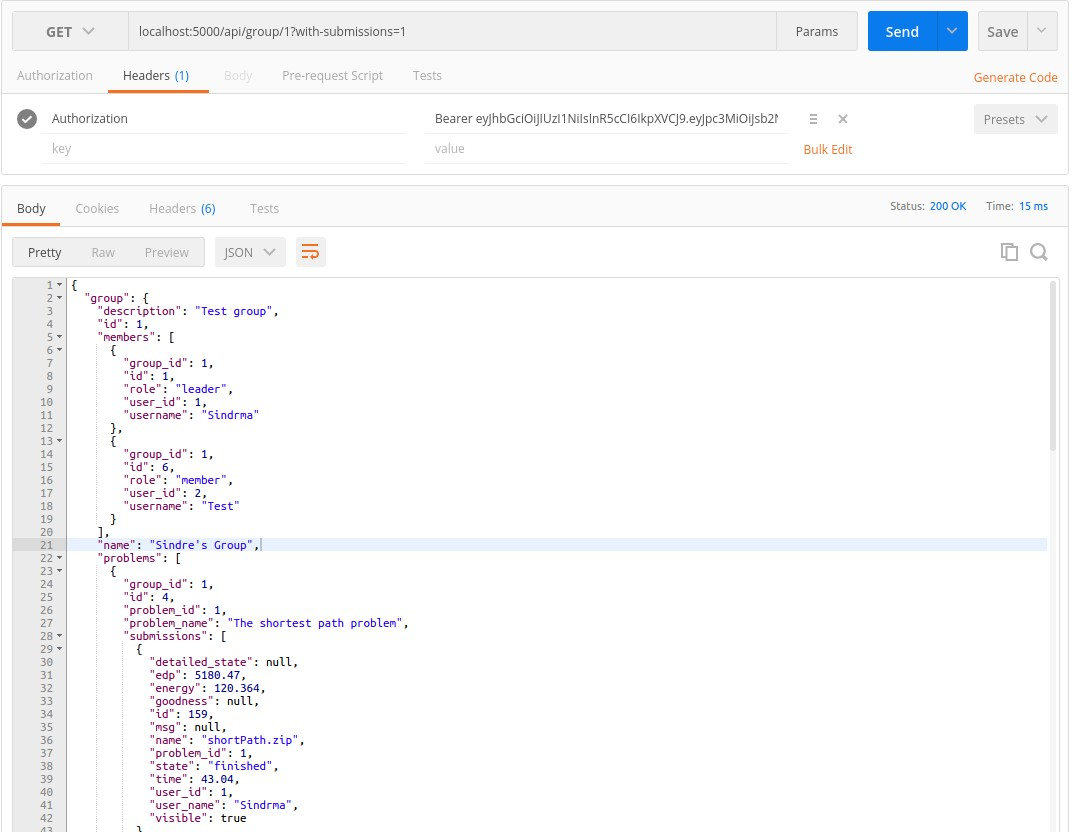
\includegraphics[width=1.0\textwidth]{figs/postman_request.jpg}
    \caption[Example request against local API]{Example request against local \gls{api} using Postman \cite{POSTMAN}. The request executes the GET-request \url{http://localhost:5000/api/group/1?with-submissions=1} presented in Table \ref{tab:cmb-updated-routes} with the query parameter \texttt{with-submissions} equal to one to also include the submissions made by the members of the group.}
    \label{fig:postman-request}
\end{figure}

\begin{table}[h!]
    \centering
    \begin{tabular}{ | c | c | p{4cm} | }
    \hline
    \textbf{\gls{api} Route} & \textbf{Method} & \textbf{Description} \\
    \hline
    \textit{/api/submission/$<$int:sub\_id$>$} & DELETE & If the submission with the given \texttt{id} exists and have been created by the current logged in user, the submission is deleted from the database as well as the file system. Requires login.\\ \hline
    \textit{/api/group/$<$int:group\_id$>$} & GET & Fetches submission information about a group by \texttt{id} depending on login status. If the user is not logged in, only public group information can be fetched. However, if the user is logged in, the user can also request information about private groups. If the query parameter \texttt{with-submissions} is set equal to 1, submissions made from group members is included in the response if the user is either a group member or leader. The response for leaders also include those submissions set to be unvisible. \\ \hline
    \textit{/api/bulletins} & GET & Returns all created bulletins. \\ \hline
    \textit{/api/bulletins/active} & GET & Returns all bulletins currently active. \\ \hline
    \end{tabular}
    \caption[\gls{cmb} API route updates with responses]{\gls{cmb} API route updates with responses. The routes listed shows the substring necessary to query the \gls{api}, and need to be combined with the \textit{path} of the server providing the \gls{api}. For example to delete a submission with \texttt{id} equal to one from the development server \gls{api}, a delete request needs to be made against \url{http://climb-dev.idi.ntnu.no/api/submission/1}.}
    \label{tab:cmb-updated-routes}
\end{table}
\clearpage
\subsection{Admin Interface}
Several new problems have been added to the system during the Spring semester. Most problems were added by the two master students assessing the \gls{cmb} system's suitability for conducting digital exams. However, during the Spring, we had a lot of trouble making the newly added problems solvable, as some submissions locked the backend infinitely. It turned out that some of the administrators had uploaded input and answer files with CR/LF (DOS) line endings, which locked the checker program during parsing of the input and answer files. The checker locked itself as the backend and server is Unix based systems and uses Unix line endings (LF). \\

The bug is removed in the new admin interface. When uploading files to the server, the files are automatically converted into Unix files with LF line endings. This is done by running all input and answer files through the \texttt{vim} \cite{VIM} command \texttt{vim + "argdo set ff=unix | update" +wqa ./*.txt} in the directory containing the problem files. The checker source file is not run through the command as the g++ compiler handles both Unix and DOS filetypes. \\

Also, some errors occurred when administrators tried to remove locked submissions in the database through the admin interface. Due to lack of training, it often left the database and the server file system in an inconsistent state. As explained above, cascading delete were added between the \texttt{Run} and \texttt{Submission} tables to partially solve the problem, but the files associated with a submission would remain in the server file system and had to be removed manually. However, deletion of submission files was often forgotten, and it caused filename conflicts if the user re-submitted zip files with equal folder and file names as a previous submission\footnote{A suggested future improvement is presented in \Cref{sec:future-work}, which is based upon storing submission files by the uniquely generated database id instead of using user defined folder and file names.}.\\

The Flask-Admin \cite{FLASKADMIN} procedure \texttt{on\_model\_delete} solves the above inconsistency problem. It has been added to handle when submissions are deleted from the database and takes care of removing all files in the server file system associated with a deleted submission. However, it is still possible to leave the database in an inconsistent state if one do not use the admin interface to delete database content. If other tools than the Flask-Admin module are to be used in the future to handle database, SQLALchemy provides event listeners which can be used instead of the above-mentioned procedure. As the \gls{cmb} team currently uses the admin interface to handle database content, the \texttt{on\_model\_delete} procedure in the Flask-Admin interface is used. \\

Administration of the Bulletin table presented in Sub-\Cref{subsec:impr-database} has also been added using the Flask-Admin module. Administration of bulletins are shown in Figure \ref{fig:admin-bulletin}, which shows how to create bulletins and how to view stored database bulletins.

\begin{figure}
    \centering
    \begin{subfigure}[b]{0.48\textwidth}
        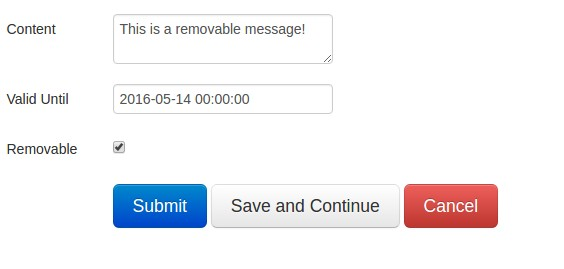
\includegraphics[width=\textwidth]{figs/bulletin_creation.jpg}
    \end{subfigure}
    ~ %add desired spacing between images, e. g. ~, \quad, \qquad, \hfill etc.
    %(or a blank line to force the subfigure onto a new line)
    \begin{subfigure}[b]{0.48\textwidth}
        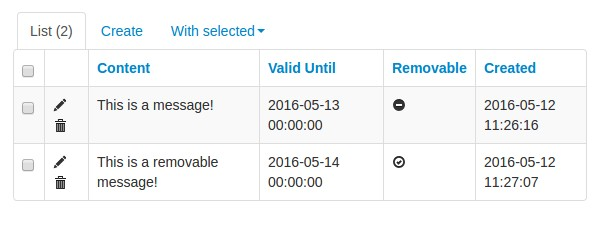
\includegraphics[width=\textwidth]{figs/bulletin_list.jpg}
    \end{subfigure}
    \caption{Bulletin creation and overview in the admin interface}
    \label{fig:admin-bulletin}
\end{figure}

\section{Backend}
\label{sec:impr-backend}
There have been some small changes in the backend code. The \gls{cmb} team discovered that there was no timeout when running the small correctness test, which could potentially lock the backend if the submitted code contained infinite loops. Locking the backend is not acceptable under any condition, and the Unix program \texttt{timeout} \cite{TIMEOUT} is therefore used during the small correctness test to kill the submitted program after some time if it halts for too long. The big correctness test already uses \texttt{timeout} to kill programs that stalls or are to slow, an the timeout is set to 90 seconds. Since the small input set is much smaller than the big correctness test, it is currently set to a third of the timeout of the big correctness. \\

The \gls{json} returned by the backend is also slightly changed. A ``state'' field were added to track the condition of the program better as it executes on the backend, especially if there is an error during execution. The field is currently used as input to the ``detailed\_state'' database field as described in \Cref{sec:impr-server}, which is further used in the frontend to specialize the feedback given to the user if there is an error during execution of the program. Currently, the field is a simple string describing the state of the submitted program when the backend are done executing, but can be extended with for example \gls{json} structures as more information about program state becomes available. A quick further discussion of the field and its potential are described in \Cref{sec:eval-tech}.

\section{Improvement Proposals}
\label{sec:impr-proposals}

\subsection{Stability Test}
An integration test\footnote{Tests multiple units or components of a system in the same test.} were developed during the Specialization project in the Autumn of 2015. The project report further described the usage of the integration test in a stability test that determined the accuracy of execution time and energy measurements over multiple submissions. A single run of the integration test sets up a test server and submits a correct solution to a problem specified by the test, by using the \texttt{nose} test framework which is, as mentioned earlier, used to develop and run unit tests. The backend and server code were also temporarily modified to output temperature readings before and after the run. A simple Bash-script was created in order to run the test multiple times with varying delay between each run of the integration test. \\

Further extending the system with an improved stability test is wanted by the \gls{cmb} team. This thesis is to propose how to further extend the stability test, as stated in objective \texttt{P1} presented in \Cref{sec:ps-inter}. The objective aims to extend the stability test by simulating synthetic workload from users. Many test frameworks makes it possible to simulate real users, but to restrict the discussion of frameworks we will only consider those which fits into the existing server code base i.e the test framework should be based on Python. Introducing frameworks dependent of other languages is not beneficial, as the \gls{cmb} system is already fairly complex and it would require a lot from future developers. It is also a great advantage if the stability test could execute automatically, for example as part of a stage in a Jenkins pipeline or in a daily executed cron job. \\

The Python based framework Funcload \cite{FUNCLOAD} is a good alternative and is used by Mozilla Services among others\footnote{See blog post: \url{http://blog.ziade.org/2013/04/25/thoughts-on-load-testing/}}. The advantage of this framework is that tests are launched through a terminal, which makes it simple to automatically launch tests and benchmarks. The frameworks offer setup of banchmarks which can simulate multiple users or clients making requests against the server, and the requests made can also transport any kind of content such as zip files. This makes it possible for the simulated users to upload and execute submissions to a problem, as in the integration test described above. The framework can also generate HTML or PDF reports after a benchmark execution, containing detailed information about the test setup, requests charts and network statistics, server CPU, load and memory usage, as well as possible failed requests. \\

Another benefit in using the Funcload framework is that it requires small changes to the existing integration test. The functionality of the Bash-script, i.e gathering data over multiple submissions, can be covered in test written in the Funcload framework as enables simulation of multiple clients. The server and backend code requires some changes in order to make the test gather data from multiple runs, and the development of the improved test should be done in correspondance with the implementation of gathering low-level statistics listed in Appendix \ref{apdx:backlog}. Results and measurement statistics such as temperature during execution should be associated with submissions made by users, and should be stored in the server file system. Under the assumption that results and statistics from runs are stored in the file system, the improved stability test should also automatically report the stability of execution time, energy, and temperature readings to cover the functionality of the previous stability test. \\

Another framework alternative is Locust \cite{LOCUST} which were also mentioned in the Specialization project report. The downside of the framework is that it sets up a web server with a web based user interface, which requires us to start the test manually through a browser. It is worth mentioning that it is possible to make the test execute through a terminal by requesting information from the Locust web-server using HTTP requests, but the framework will still setup a web-server which seems to be a little drastic compared to our simple requirements. However, the web interface is simple to use and is also very popular on GitHub. \\

Both frameworks mentioned above requires a running \gls{cmb} server and backend to work. The previous integration test only required a running backend as the test automatically started a test server, and it should be explored if it is possible to do the same with the introduction of one of the above frameworks to follow the testing standard in the project. Another alternative is to run the stability test on a designated server which is a true copy of the production server, which is used by few real users. The introduction of a new designated production like test server is discussed further in \Cref{sec:future-work} as possible future development.

\subsection{How-To Page and About Page}
The user feedback from TDT4200 \cite{TDT4200} pointed out that HowTo-page were unclear on how to structure the content of zip files to be uploaded. Some users also reported that it would be nice with an explanation of Unix error codes, which is presented to users if their submission terminates with an run time error. In addition, a solution to the OSX upload bug were discovered during the Spring and has been implemented as explained in \Cref{sec:impr-frontend}. However, if OSX users still experiences problems, an explanation of how to correctly create a zip on OSX systems should be added to the HowTo page. As the system were to be used in experiments in the course TDT4102 \cite{TDT4102} and in the user test presented in \Cref{sec:user-testing}, the HowTo page were updated with the above information. \\

The page should also be further extended as the system is extended with more features. There is also some small possible extensions which can be made to improve the content on the HowTo-page. Among the things missing is examples if input and output code samples in C, as the current page only has an example of C++ code IO handling. The text explaining the uploads can also be further extended with a descriptive figure to make it even more clear how to upload code to the current system. The HowTo could also contain a FAQ, which can be updated as questions are reported by users. \\

Another idea apart from the HowTo page is to add an About page. The About page should describe the project and system in an easy way, as well as describing the motivation and purpose of the project and system. The page should also explain technical aspects, such as an explanation of \gls{edp} which may be an unknown metric for programmers new to energy efficient metrics. A list of publications related to the system would also be nice. The About page was not added to the system in this thesis.

\subsection{Adding Problems}
This thesis has not contributed towards adding new problems. However, all problems used in the \gls{cmb} system is advised to follow the standard of problems present in other \glspl{oj}. Some of the \glspl{oj} mentioned in \Cref{sec:related} are used in \gls{icpc} programming competitions, and seems to follow the same format in their provided problem descriptions. The \gls{cmb} system should aim to offer problems following a similar format, as the system may be used in similar competitions in the future. The \gls{cmb} team should also strive to add more problems, hopefully with as much diversity as offered by other \glspl{oj}.

\subsection{Discussion Forum}
A discussion forum is wanted by the \gls{cmb} team. There exist multiple third party solutions offering online forums which offers varying degrees of modifiability, and we here restrict the discussion of third party solutions by requiring that the software is related to technologies used in the system or is known by the \gls{cmb} team. The framework FlaskBB \cite{FLASKBB} is a Python Flask based lightweight forum module, and seems to offer some degree of modifiability. The framework offers simple forum functionality such as posting questions, issue tracking, private messages, and forum administration. It is also possible to create own themes to better match the frontend view. There is also a popular Javascript based open-source forum software called Flarum \cite{FLARUM}, which offers much the same features as FlaskBB. It is also worth mentioning that third party software like Piazza is an option, but future developers should keep in mind that the software offers only small modifications of its appearance. \\

A deeper study should be conducted before choosing how to implement a discussion forum. To make the system look more professional, a third party module with a highly modifiable appearance should be chosen. Another possibility is to build the forum software from scratch. A con is that it takes a lot of time to develop forum software, but a benefit is that no new software needs to be introduced in order to develop the forum and it makes the system look more professional to the outside world.
